%%%%%%%%%%%%%%%%%%%%%%%%%%%%%%%%%
%
% Lecture notes for Numerical Methods for Partial Differential Equations
%
% Chapter 2: Parabolic PDEs
%   Sections 1 and 2
%
%%%%%%%%%%%%%%%%%%%%%%%%%%%%%%%%%

% !TeX root = NumPDE_Lecture_notes.tex

\section{Parabolic partial differential equations}

\subsection{Explicit finite-difference method for the heat equation}
 
We will illustrate the finite-difference
methods for parabolic PDEs with the heat, or diffusion, equation
\begin{equation}\label{a1}
\frac{\pr u}{\pr t}(x,t) = K\frac{\pr^{2} u}{\pr x^{2}}(x,t), \quad
0<x< L, \quad 0 < t < T,
\end{equation}
subject to the Neumann boundary conditions
\begin{equation}\label{a2}
u(0, t) = u(L, t)=0 \quad \hbox{for} \quad t\in (0,T),
\end{equation}
and the initial condition
\begin{equation}\label{a3}
u(x, 0) = u_{0}(x),
\end{equation}
where $u_{0}(x)$ is a given function. In Eq. \eqref{a1}, $K$ is a positive
constant.
In what follows, we assume that (i) the initial condition \eqref{a3} is consistent with
the boundary conditions (\ref{a2}) (i.e. $u_{0}(0)=u_{0}(L)=0$), (ii) $u_{0}(x)$ is twice differentiable in $x$ on $[0,L]$ and (iii) a unique solution of the initial boundary-value problem (\ref{a1})--(\ref{a3}) exists.
 
First we choose integers $N$ and $M$ and define
$h$ and $\tau$ as
\[
\tau=\frac{T}{M}, \quad h=\frac{L}{N}.
\]
Then we define the grid points (or mesh points)
$(x_{k}, t_{j})$, where $x_{k}=hk$ for $k=0,1,\dots,N$ and
$t_{j}=\tau j$ for $j=0,1,2,\dots,M$. The problem is to find numbers $w_{kj}$
(for $k=0,1,\dots,N$ and $j=0,1,2,\dots$) such that $w_{kj}$ approximates the value of the exact solution
$u(x,t)$ at the grid point $(x_{k}, t_{j})$.
\begin{figure}[h]
\centering

\includegraphics[width=11cm,height=8cm]{basic_grid2.pdf}
\caption{}
\end{figure}
 
To obtain a finite-difference method, we need to approximate the partial derivatives
with respect to $t$ and $x$ at the grid points. By definition,
the partial derivative of the function $u(x,t)$ with respect to
$t$ at point $(x_k,t_j)$ is
\[
\frac{\pr u}{\pr t}(x_k,t_j)=\lim_{\tau\to 0}\frac{u(x_k,t_j+\tau)-u(x_k,t_j)}{\tau}.
\]
It is natural to expect that
\begin{equation}
\frac{\pr u}{\pr t}(x_k,t_j)\approx \frac{u(x_k,t_j+\tau)-u(x_k,t_j)}{\tau}
\label{a10}
\end{equation}
for sufficiently small $\tau$. What is the error of this formula?
To find this, we assume that $u$ is sufficiently smooth (so that its first and second
derivatives with respect to $t$ are continuous in the interval $(0,T)$ for some $T>0$)
and write the first Taylor polynomial for $u(x_k,t_j+\tau)$:
\[
u(x_k,t_j+\tau)=u(x_k,t_j)+\tau \frac{\pr u}{\pr t}(x_k,t_j)+
\frac{\tau^2}{2}\frac{\pr^2 u}{\pr t^2}(x_k,\xi)
\]
where $\xi$ is between $t_j$ and $t_j+\tau$. It follows that the error,
which is called the {\bf truncation error } and denoted by $\tau_{kj}$,
is given by
\[
\tau_{kj}=\frac{\pr u}{\pr t}(x_k,t_j)-\frac{u(x_k,t_j+\tau)-u(x_k,t_j)}{\tau}=
-\frac{\tau}{2}\frac{\pr^2 u}{\pr t^2}(x_k,\xi).
\]
Thus, if $\frac{\pr^2 u}{\pr t^2}(x,t)$ is bounded for all $x$ and $t$, then
\[
\tau_{kj}=O(\tau).
\]
Formula (\ref{a10}) with $\tau>0$ is called the {\bf forward-difference formula}
for the first derivative.
If in (\ref{a10}) we replace $\tau$ by $-\tau$, we obtain the formula
\begin{equation}
\frac{\pr u}{\pr t}(x_k,t_j)\approx \frac{u(x_k,t_j)-u(x_k,t_j-\tau)}{\tau},
\label{a11}
\end{equation}
which is called the {\bf backward-difference formula} (for the first derivative).
 
To derive a finite difference formula for $\pr^2 u(x_k,t_j)/\pr x^2$, we first write the Taylor series expansions
of $u(x_k+h,t_j)$ and $u(x_k-h,t_j)$ at the point $(x_k,t_j)$:
\begin{eqnarray*}
u(x_k+h,t_j)=u(x_k,t_j)&+&h \frac{\pr u}{\pr x}(x_k,t_j)+
\frac{h^2}{2}\frac{\pr^2 u}{\pr x^2}(x_k,t_j)\\
&+&\frac{h^3}{6}\frac{\pr^3 u}{\pr x^3}(x_k,t_{j})+
\frac{h^4}{24}\frac{\pr^4 u}{\pr x^4}(\xi_1,t_{j}), \\
u(x_k-h,t_j)=u(x_k,t_j)&-&h \frac{\pr u}{\pr x}(x_k,t_j)+
\frac{h^2}{2}\frac{\pr^2 u}{\pr x^2}(x_k,t_j)\\
&-&\frac{h^3}{6}\frac{\pr^3 u}{\pr x^3}(x_k,t_{j})+
\frac{h^4}{24}\frac{\pr^4 u}{\pr x^4}(\xi_2,t_{j}) 
\end{eqnarray*}
for some $\xi_{1}$ between $x_{k}$ and $x_{k}+h$
and some $\xi_{2}$ between $x_{k}-h$ and $x_{k}$. 
The sum of these equations gives us the formula
\begin{multline}
u(x_k+h,t_j)+u(x_k-h,t_j)=2u(x_k,t_j)+ h^2\frac{\pr^2 u}{\pr
x^2}(x_k,t_j)\\
+ \frac{h^4}{24}\left(\frac{\pr^4 u}{\pr
x^4}(\xi_1,t_{j}) +\frac{\pr^4 u}{\pr x^4}(\xi_2,t_{j})\right).
\end{multline}
If $\pr^4 u(x,t)/\pr x^4$ is continuous, we can write this in a more compact form. Indeed, the number
\[
\frac{1}{2}\left(\frac{\pr^4 u}{\pr x^4}(\xi_{1}, t_{j})+\frac{\pr^4 u}{\pr x^4}(\xi_{2},t_{j})\right)
\]
is between
the numbers $\frac{\pr^4 u}{\pr x^4}(\xi_{1},t_{j})$ and $\frac{\pr^4 u}{\pr x^4}(\xi_{2},t_{j})$. Therefore,
by the intermediate value theorem, there is a number $\xi$ between $\xi_{1}$ and $\xi_{2}$ such that
$\frac{1}{2}\left(\frac{\pr^4 u}{\pr x^4}(\xi_{1},t_{j})+\frac{\pr^4 u}{\pr x^4}(\xi_{2},t_{j})\right)
=\frac{\pr^4 u}{\pr x^4}(\xi,t_{j})$. Therefore, we obtain
\begin{equation}
\frac{\pr^2 u}{\pr x^2}(x_k,t_j)=\frac{u(x_{k+1},t_j)-2u(x_k,t_j)+u(x_{k-1},t_j)}{h^2}
-\frac{h^2}{12}\frac{\pr^4 u}{\pr x^4}(\xi,t_{j}), \label{a17}
\end{equation}
where $\xi$ is a number between $x_{k}-h$ and $x_{k}+h$.
This is called the {\bf central difference formula} for $u_xx$. When $u_{xxxx}$ is bounded,
then the truncation error in the central difference approximation is $O(h^2)$.
  
 
Now we are ready to obtain the finite-difference equations that approximate
the heat equation (\ref{a1}). First, we introduce numbers $w_{kj}$ for $k=0,1,\dots,N$ and
$j=0,1,2,\dots$ that approximate the exact solution $u(x,t)$ of Eq. (\ref{a1}) at the grid points
$(x_{k}, t_{j})$:
\[
w_{kj}\approx u(x_{k},t_{j}).
\]
Then, we use Eqs. (\ref{a10}) and (\ref{a17}) to approximate
the corresponding derivatives in the heat equation. As a result we obtain the following
difference equations
\begin{equation}
\frac{w_{k,j+1}-w_{kj}}{\tau}-K
\frac{w_{k+1, j}-2w_{kj}+w_{k-1,j}}{h^{2}}=0, \label{b4}
\end{equation}
for each $k=1, 2, \dots, N-1$ and $j=0, 1, \dots, M-1$. Equation ({\ref{b4})
which approximates our PDE at point $(x_{k},t_{j})$ uses approximations to the solution
not only at this point but also
at three neighbouring points $(x_{k+1},t_{j})$, $(x_{k-1},t_{j})$ and $(x_{k},t_{j+1})$.

In approximating the heat equation by the difference equation \eqref{b4} we
introduced a truncation error of from approximating the $t$ derivative of $O(\tau)$
and another truncation error from approximating the $x$ derivative of $O(h^2)$.
Thus it is natural to expect that the truncation error in the difference
equation \eqref{b4} is of order $O(\tau)+O(h^2)$. However we will meet more 
complicated finite-difference methods where the errors do not simply add, so
we need a proper definition of what we mean by the truncation error of a 
finite-difference approximation.

\begin{definition}
Let us represent a PDE as $D\,u=0$, where $D$ is a differential operator,
and the corresponding difference equation as $D_{f.d.}\,w=0$, where
$D_{f.d.}$ is the finite-difference operator that approximates $D$. Then
the {\bf local truncation error} $\tau_{kj}$ of the finite-difference 
approximation at grid point $(x_k,t_j)$ is 
\[\tau_{kj}=(D_{f.d.}\,u)_{kj},\]
i.e., it is equal to the value of the left hand side of the difference
equation evaluated on the exact solution of the differential equation.
\end{definition}
The local truncation error of
the difference equation (\ref{b4}) is given by
\begin{eqnarray*}
\tau_{kj} &=& (D_{f.d.}\,u)_{kj} =
\frac{u_{k,j+1}-u_{kj}}{\tau}-K
\frac{u_{k+1, j}-2u_{kj}+u_{k-1,j}}{h^{2}} \\
&=& \frac{\pr u}{\pr t}(x_{k},t_{j})-
K\frac{\pr^2 u}{\pr x^2}(x_{k},t_{j})+
\frac{\tau}{2}\frac{\pr^{2} u}{\pr t^{2}}(x_{k},
\xi_{1})- K\frac{h^{2}}{12}\frac{\pr^{4} u}{\pr x^{4}}(\xi,t_{j})\\
&=&\frac{\tau}{2}\frac{\pr^{2} u}{\pr t^{2}}(x_{k},
\xi_{1})- K\frac{h^{2}}{12}\frac{\pr^{4} u}{\pr x^{4}}(\xi,t_{j})\\
&=&O(\tau)+O(h^{2})=O(\tau+h^{2}). 
\end{eqnarray*}
Here we used the notation $u_{kj}=u(x_{k}, t_{j})$. 
So in this case the local truncation error is just the sum of the truncation error
from the finite-difference approximation for the time derivative and
the truncation error from the finite-difference approximation for the space
derivative, as we expected.

Equation (\ref{b4}) can be written as
\begin{equation}
w_{k,j+1}=\left(1-2\gamma\right)w_{kj}+
\gamma\left(
w_{k+1, j}+w_{k-1,j}\right), \label{b5}
\end{equation}
for $k=1,\dots,N-1$ and
$j=0,1,\dots, M-1$. In Eq. (\ref{b5}),
$\gamma\equiv K\tau/h^{2}$. Since the initial condition $u(x,0)=u_{0}(x)$
implies that $w_{k,0}=u_{0}(x_{k})$ for each $k=0, 1, \dots, N$, these values can be used in
Eq. (\ref{b5}) to find the value of $w_{k,1}$ for each $k=1, 2, \dots, N-1$. The boundary conditions
$u(0,t)=u(l,t)=0$ imply that $w_{0,1}=w_{N,1}=0$. Now we know $w_{k,1}$ for each $k=0,1,\dots, N$.
Then the same procedure is applied to find $w_{k,2}$, $w_{k,3}$, etc.


 
 
The method described above is called the {{\bf forward-difference method}.
It can also be written in the matrix form
\begin{equation}
{\bf w}^{(j)}=A{\bf w}^{(j-1)} \quad \hbox{for} \quad j=1,2,\dots, \label{b6}
\end{equation}
where
\begin{equation}
A=\left[
\begin{array}{cccccc}
1-2\gamma &\gamma &0      &\dots  &\dots &0 \\
\gamma &1-2\gamma &\gamma &\ddots  &     &\vdots \\
0      &\gamma &1-2\gamma &\gamma &\ddots &\vdots \\
\vdots &\ddots &\ddots &\ddots &\ddots &0 \\
\vdots &       &\ddots &\ddots &\ddots &\gamma \\
0      &\dots  &\dots  &0      &\gamma &1-2\gamma
\end{array}\right], \quad
{\bf w}^{(j)}=\left[
\begin{array}{c}
w_{1,j} \\
w_{2,j} \\
\vdots \\
\vdots \\
\vdots \\
w_{N-1,j}
\end{array}\right].
\label{b7}
\end{equation}
The forward-difference method for the heat equation is an example of an {\bf explicit finite-difference method}.
It is explicit because we do not need to solve any equations, we just use the explicit formula (\ref{b6}).
\begin{figure}[h]
\centering
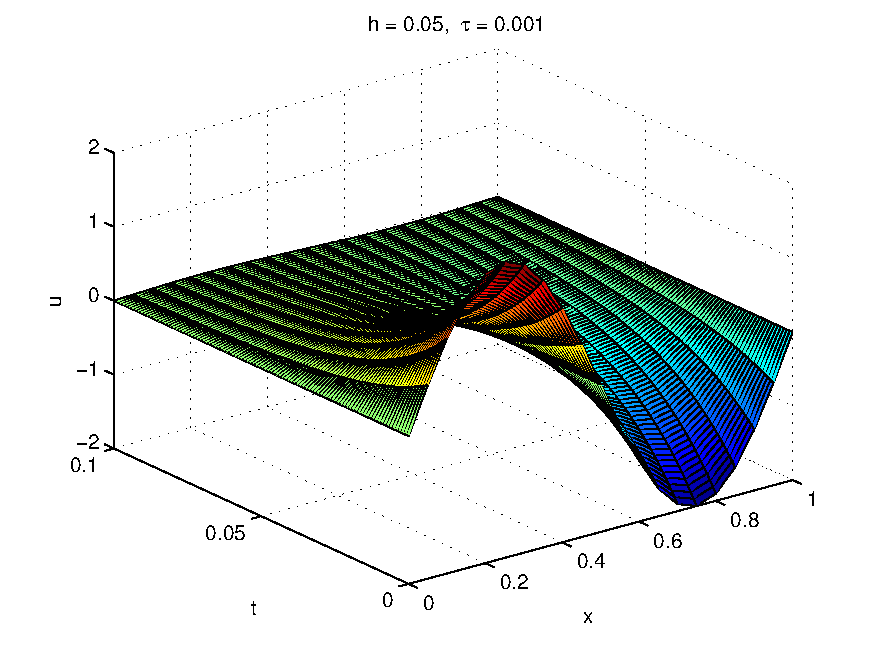
\includegraphics[width=11cm,height=8cm]{forward_diff_fig1.pdf}
\caption{Solution of the forward-difference approximation of the heat equation 
\eqref{a1} with boundary condition \eqref{a2} and initial condition $u(x,0)=2\sin(2\pi x)$ for
$K=1$ and $t\in[0,0.1]$. Step sizes are $h=0.05$ and $\tau=0.001$.}
\label{fig2}
\end{figure}

\begin{figure}[h]
\centering
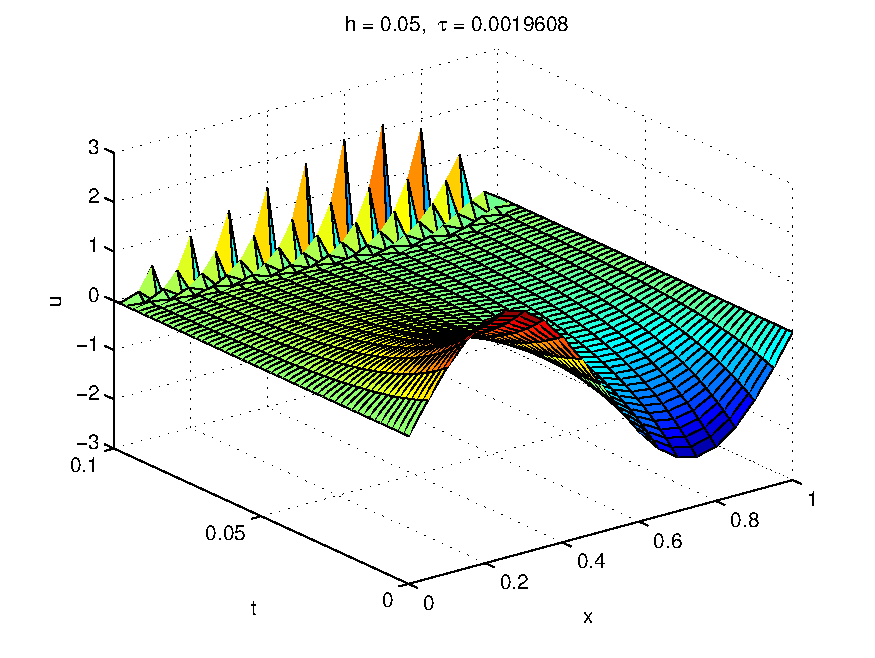
\includegraphics[width=11cm,height=8cm]{forward_diff_fig2.pdf}
\caption{Solution of the forward-difference approximation for the same
equation as in Figure \ref{fig2} but with step sizes are $h=0.05$ and $\tau=0.1/51$.}
\label{fig3}
\end{figure}
A surface plot of the solution $u(x,t)$ of problem (\ref{a1})--(\ref{a3}) for $L=1$, $T=0.1$
and $u_{0}(x)=2 \sin(2\pi x)$, obtained with the help of the forward-difference
method, is shown in Figure \ref{fig2}. So, the method works!

Will it always work? It turns out that it doesn't work if the time step $\tau$ is not small enough.
For example, if we solve the same problem on a grid with a bigger $\tau$, we get what is shown in Figure \ref{fig3}.
So, in this case, the forward-difference method doesn't work properly. The reason for this is that
the finite-difference scheme becomes \textbf{unstable} when $\tau$ is not sufficiently small.


%%%%%%%%%%%%%%%%%%%%%%%%%%%%%%%%%%%%%%%%%%%%%%%%%%%%%%%%%%%%%%%%%%%%%%%%%%%%%%%%

\subsection{Stability}

 
If there are errors $z_{10},
z_{20},\dots, z_{N-1,0}$ in the initial data $w_{10},w_{20},\dots,
w_{N-1,0}$ (or at any particular step, the choice of the initial
step is simply for convenience), the errors propagates to
$w_{11},w_{21},\dots, w_{N-1,1}$, then to 
\linebreak[4]$w_{12},w_{22},\dots,
w_{N-1,2}$, etc. If the errors grow with each time step, then the
difference method in unstable. If they do not grow, it is stable.
How to find out whether a finite-difference method is stable?

Let ${\bf z}^{(0)}=(z_{1}^{(0)}, z_{2}^{(0)},\dots, z_{N-1}^{(0)})^{T}$
be the initial error (or perturbation). Then it follows from (\ref{b6})
that
\[
\tilde{\bf w}^{(1)}=A\tilde{\bf w}^{(0)}=A\left({\bf w}^{(0)}+{\bf z}^{(0)}\right)=A{\bf w}^{(0)}+A{\bf z}^{(0)},
\]
i.e.
\[
{\bf z}^{(1)}=\tilde{\bf w}^{(1)}-{\bf w}^{(1)}=A{\bf z}^{(0)}.
\]
At the $n$-th time step, the error in $\tilde{\bf w}^{(n)}$
due to ${\bf z}^{(0)}$ is ${\bf z}^{(n)}=A^{n}{\bf z}^{(0)}$.
The method is stable if these errors do not grow as $n$ increases, i.e. if and only if
for any initial error ${\bf z}^{(0)}$ we have $\Vert A^{n}{\bf z}^{(0)}\Vert\leq \Vert {\bf z}^{(0)}\Vert$
for all $n$ or, equivalently, $\Vert A{\bf z}^{(0)}\Vert\leq \Vert {\bf z}^{(0)}\Vert$ (here $\Vert\cdot\Vert$
is any vector norm). This, in turn, is
equivalent to the condition that magnitudes of all eigenvalues of $A$ are equal to or smaller than 1,
i.e.
\[
\vert\lambda_{i}\vert\leq 1 \quad \hbox{for} \quad i=1, 2, \dots, N-1.
\]
So, to solve the stability problem we need to calculate the eigenvalues of $A$. 

Calculating the eigenvalues of the matrix in eq.\eqref{b7} analytically is a bit hard.
Instead, we will consider the problem with the boundary conditions
\eqref{a2} replaced by periodic boundary conditions
\begin{equation}
u(x,0)=u(x,L).
\end{equation}
In most cases the stability will not be affected much by this change in boundary
condition. Physically the heat equation with this periodic boundary condition 
would model the heat of a circular rod, where heat flowing out of the right
end flows back in at the left end.

The periodic boundary condition implies that at the boundary point
$k=N$ we have the same value as at $k=0$, but this value is no longer fixed.
Instead we have to use equation \eqref{b5} also for the boundary point $k=N$, 
with the convention that $k=N+1$ is identified with $k=1$. Therefore
eq. \eqref{b7} gets replaced by
\begin{equation}
A=\left[
\begin{array}{cccccc}
1-2\gamma &\gamma &0      &\dots  &0 &\gamma \\
\gamma &1-2\gamma &\gamma &\ddots  &\vdots &0\\
0      &\gamma &1-2\gamma &\gamma &\ddots &\vdots \\
\vdots &\ddots &\ddots &\ddots &\ddots &0 \\
0 &       &\ddots &\ddots &\ddots &\gamma \\
\gamma      &0  &\dots  &0      &\gamma &1-2\gamma
\end{array}\right], \quad
{\bf w}^{(j)}=\left[
\begin{array}{c}
w_{1,j} \\
w_{2,j} \\
\vdots \\
\vdots \\
\vdots \\
w_{N,j}
\end{array}\right].
\label{bp7}
\end{equation}
Luckily this matrix is a
circulant matrix, where each row is equal to the row above, just circularly
shifted to the right by one. 
The eigenvectors of such a matrix are of the form
\[{\bf v} = (1,z,z^2,\dots,z^{N-1})\]
where $z$ is any of the $N$-th roots of unity, $z=\exp(2\pi i n)$ for $n=1,\dots,N$. This knowledge of the
eigenvectors of course makes it simple to calculate the eigenvalues
of the matrix $A$ simply by acting with $A$ on each of the eigenvectors.

Because the matrix for periodic boundary conditions differs from the matrix
for Neumann boundary conditions only in two places, it is plausible that
the eigenvalues will also not differ much between the two cases.

We can also do the stability analysis with periodic boundary conditions
without first writing down
the matrix $A$ but instead directly solving the difference equations. We
refer to this approach as the {\bf Fourier method}.
Let $w_{kj}$ be the exact solution of the difference equation (\ref{b4})
\begin{equation}
\frac{w_{k,j+1}-w_{k,j}}{\tau}-K\frac{w_{k+1,j}-2w_{k,j}+w_{k-1,j}}{h^2}=0 \label{b15}
\end{equation}
(the forward-difference method).
The initial data
\[
z_{k,0}=\tilde{w}_{k,0}-w_{k,0}=\tilde{w}_{k,0}-u_{0}(x_{k}) \quad
\hbox{for} \quad k=0, 1, \dots, N,
\]
propagates with each step in time resulting in another
solution of $\tilde{w}_{kj}$. Let
$z_{kj}=\tilde{w}_{kj}-w_{kj}$ be the error at the mesh point
$(x_{k}, t_{j})$ for each $k=0,1,2, \dots, N$ and $j=0,1, \dots, M$.  $z_{kj}$ satisfies the difference
equation
\begin{equation}
\frac{z_{k,j+1}-z_{k,j}}{\tau}-K\frac{z_{k+1,j}-2z_{k,j}+z_{k-1,j}}{h^2}=0 \label{b16}
\end{equation}
for $k=1,2, \dots, N$ and $j=0,1,\dots,M-1$. (Note that Eq.
(\ref{b16}) coincides with (\ref{b4}). This is because Eq. (\ref{b4}) is linear and homogeneous.) In the Fourier method, we seek a particular solution of
(\ref{b16}) in the form
\begin{equation}
z_{k,j}=\rho_{q}^{j}e^{iqx_{k}}, \quad q\in{\mathbb R}. \label{b17}
\end{equation}
(Here $i=\sqrt{-1}$.) Then the finite-difference method (\ref{b4})
is stable, if all solutions having the form (\ref{b17}) are such that
\[
\vert\rho_{q}\vert\leq 1
\]
for all $q\in{\mathbb R}$.

\vskip 3mm  
Substitution of (\ref{b17}) into (\ref{b16})
yields
\[
\frac{\rho_{q}^{j+1}e^{iqx_{k}}-\rho_{q}^{j}e^{iqx_{k}}}{\tau}-
K\frac{\rho_{q}^{j}\left(e^{iqx_{k+1}}-2e^{iqx_{k}}+e^{iqx_{k-1}}\right)}{h^2}=0
\]
or
\[
\rho_{q}-1 - \gamma \left(e^{iqh}-2+e^{-iqh}\right)=0.
\]
Since
\[
e^{iqh}-2+e^{-iqh}=\left(e^{iqh/2}-e^{-iqh/2}\right)^{2}=-4\sin^{2}
\frac{qh}{2},
\]
we obtain
\[
\rho_{q}=1-4\gamma\sin^{2} \frac{qh}{2}.
\]
The method is stable if
\[
\left\vert 1-4\gamma\sin^{2}\frac{qh}{2}\right\vert\leq 1
\]
for each $q$, which is equivalent to
\[
-1\leq 1-4\gamma\sin^{2}\frac{qh}{2}\leq 1 .
\]
This double inequality is satisfied provided that
\[
0\leq \gamma\sin^{2}\frac{qh}{2}\leq \frac{1}{2}.
\]
Evidently, the last inequality holds for all $q$ if
\begin{equation}
0\leq\gamma \leq \frac{1}{2} \quad \text{ or equivalently} \quad0\leq \tau \leq
\frac{h^2}{2K}. \label{aa}
\end{equation}
Thus, we arrive at the conclusion that the forward-difference method is
stable only if (\ref{aa}) is satisfied.

\vskip 3mm   A method which is stable only if a certain
condition holds is called {\bf conditionally stable}. Thus, the
forward-difference method for the heat equation is conditionally
stable.

